\documentclass{ou-report-vaf}
\citestyle{agu}

% -------------------- Packages --------------------
\usepackage{graphicx}
\usepackage{tikz}
\usepackage{pgfgantt}
\usepackage{booktabs}

% -------------------- Title metadata --------------------
\title[Research Proposal]{Requirements Traceability for Scriptless GUI Testing}
\author{R.\ J.\ H.\ van de Wetering}

\begin{document}

% ==================== Title page ====================
\begin{titlepage}
    \thispagestyle{empty}
    \begin{center}
        % Logo
        \begin{tikzpicture}[remember picture,overlay]
            \node[anchor=south, inner sep=0pt] at (current page.south) {
\includegraphics[scale=0.7]{logo}};
        \end{tikzpicture}
    
        \vspace*{2\bigskipamount}

        % Title
        {\makeatletter
            \titlestyle\color{title}\Huge\@title
        \makeatother}
    
        % Optional subtitle
        {\makeatletter
            \ifx\@subtitle\undefined\else
                \bigskip
                \titlefont\titleshape\LARGE\@subtitle
            \fi
        \makeatother}
    
        \vspace{2\bigskipamount}
        by
        \vspace{2\bigskipamount}
    
        % Author
        {\makeatletter
            \titlefont\Large\bfseries\@author
        \makeatother}
        
        \vspace{4\bigskipamount}

        % Metadata
        \begin{tabular}{lll}
            Student number:     & 852337023 \\
            Course code:        & \textsc{IM}9703 \\
            Thesis committee:   & Prof.\ dr.\ T.\ E.\ J.\ Vos (chair),  & Open University \\
                                & Dr.\ F.\ P.\ Ric\'os (supervisor),    & Polytechnic University of Valencia \\
        \end{tabular}
    \end{center}
\end{titlepage}

% ==================== Front matter ====================
\pagenumbering{roman}
\pagestyle{plain}

\setcounter{tocdepth}{2}
\tableofcontents

\clearpage

% ==================== Main matter ====================
\pagenumbering{arabic}
\let\cleardoublepage\clearpage

% ====================================================
% Introduction
% ====================================================
\section{Introduction}
\label{sec:introduction}

Automated scriptless testing explores software without predefined test scripts, which drastically reduces maintenance while allowing more unexpected behavior to be found. TESTAR is an open-source scriptless testing tool that performs automated graphical user interface (GUI) exploration by detecting available widgets, performing interactions, and traversing the System Under Test (SUT) without human-made test cases~\citep{vos2021testar}. Through this exploration, TESTAR can expose failures such as crashes, freezes, and unexpected screens without requiring access to the codebase. TESTAR supports several exploration strategies, including random selection, Q-learning, genetic algorithms, and more recent approaches driven by large language models (LLM)~\citep{esparcia2016q,esparcia2018using,van2025llm}. Unlike random and learning-based exploration that primarily optimizes coverage or reward, LLM-guided strategies can steer TESTAR’s interactions in a more goal-directed manner by selecting actions that more consistently advance specific functional test goals.

During exploration, TESTAR stores the observed widgets, actions, states, and transitions in a graph structure called the GUI State Model. These models, stored in the OrientDB multi-model graph database, provide a detailed representation of the observed GUI behavior and support offline analysis of failures (e.g., via offline oracles)~\citep{de2019offline} as well as GUI change detection across software versions~\citep{ricos2025delta}.

However, GUI State Models do not align well with the functional perspectives that are typically used in software development. Organizations reason in terms of user stories, workflows, and functional requirements, whereas TESTAR produces low-level GUI action sequences. As a result, stakeholders such as product owners cannot readily see which user stories have been executed, whether they were completed, or which functional processes were covered by scriptless tests.

This disconnect limits traceability between automated scriptless testing and the functional specifications used in software development. Improving this traceability would make scriptless testing tools like TESTAR more useful to stakeholders by interpreting exploratory behavior in terms of functional requirements and user story coverage. Bridging this gap between functional specifications and observed GUI interactions forms the core problem of this research. An illustration of the disconnect is shown in Figure~\ref{fig:intro-illustration}.

\begin{figure}[h!tb]
    \centering
    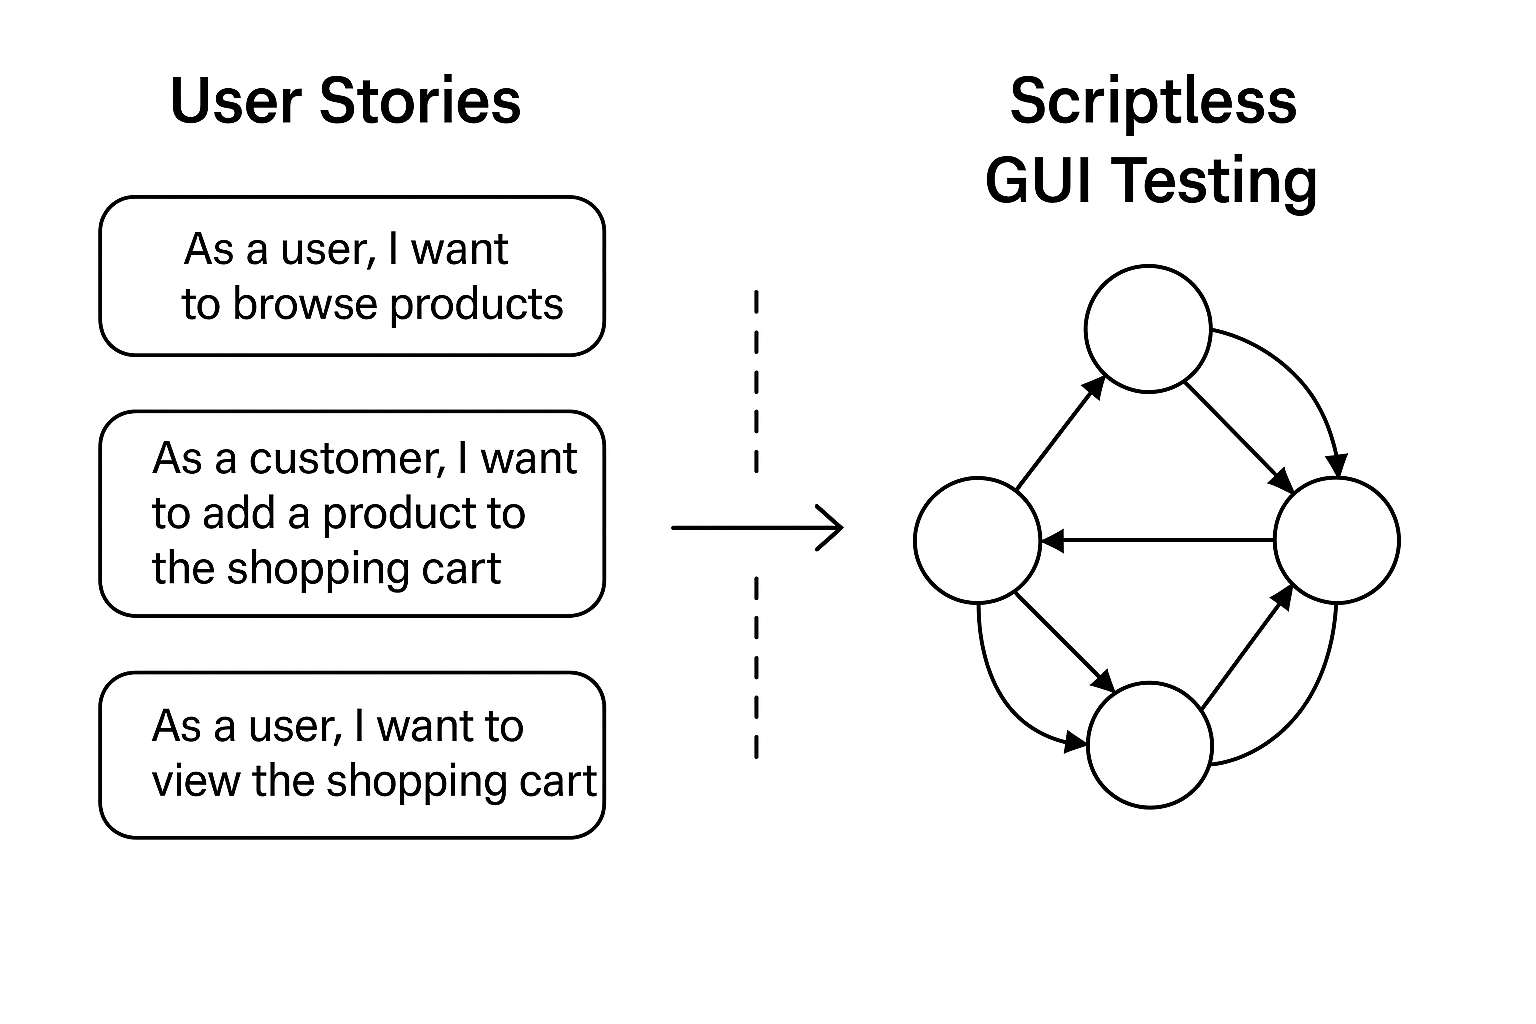
\includegraphics[width=0.6\textwidth]{intro_illustration.png}
    \caption{The gap between user stories and scriptless GUI testing.}
    \label{fig:intro-illustration}
\end{figure}

\clearpage
% ====================================================
% Related Work
% ====================================================
\section{Related Work}
\label{sec:relatedwork}

This section reviews prior work on scriptless testing and GUI State Models, user stories as requirements artifacts, and requirements traceability, and identifies the gap addressed by this research.

\subsection{Scriptless GUI Testing and GUI State Models}
\label{subsec:scriptless-gui-models}

Scriptless GUI testing tools execute applications without predefined test cases and infer behavior directly through interaction. Earlier work on model-based GUI testing investigated how event-flow graphs and widget hierarchies can support automated test generation and coverage analysis~\citep{memon2007event}. TESTAR continues this line of research by dynamically exploring applications and recording observed behavior in graph-based structures known as \emph{GUI State Models}~\citep{vos2021testar}. These models capture the states encountered during exploration, the actions available within each state, and the transitions triggered by interacting with GUI elements.

Because scriptless exploration may traverse diverse and unpredictable interaction paths, the resulting GUI State Models often become extensive and highly interconnected. Prior research illustrates this tendency: \citet{mulders2022state} show that GUI state spaces grow rapidly during run-time test generation, requiring abstraction mechanisms to control model complexity, while \citet{ricos2023distributed} demonstrate that inferring complete models for larger systems can be computationally demanding enough to require distributed processing. Such complexity makes GUI State Models valuable for fault detection, regression analysis, and behavioral comparison across software versions. However, it also renders them impractical for stakeholders attempting to reason about functional behavior: the models encode low-level GUI events and transitions, whereas stakeholders work with higher-level specifications such as user stories. Consequently, manually determining which user stories were executed and whether they were completed would be extremely time-consuming and practically infeasible.

Figure~\ref{fig:gui-state-model} illustrates a typical GUI State Model. While such representations effectively capture operational GUI behavior, they do not correspond directly to functional specifications. This mismatch between low-level interaction models and high-level functional descriptions forms a central component of the traceability challenge addressed in this research.

\begin{figure}[h!tb]
    \includegraphics{gui-state-model.png}
    \caption{Example of a GUI State Model.}
    \label{fig:gui-state-model}
\end{figure}

\subsection{User Stories and Scenario Representation}
\label{subsec:user-stories}

User stories are widely used in agile development to express functional requirements from a stakeholder perspective. A user story typically follows the Connextra template popularized by Cohn: ``As a <role>, I want <goal> so that <reason>'', which emphasizes user intent rather than system mechanics~\citep{cohn2004user}. While this format is deliberately lightweight and flexible, its natural-language form complicates automated interpretation and tool-supported analysis.

To address this challenge, researchers have proposed methods for improving the clarity and analyzability of user stories. \citet{lucassen2016improving} introduced the Quality User Story (QUS) framework, providing criteria such as atomicity, unambiguity, and conceptual consistency, to help transform user stories into more structured and analyzable units. Further work in requirements engineering explores natural-language processing (NLP) techniques to identify actors, actions, and scenario flows within user stories, enabling the extraction of semi-structured representations suitable for automated analysis~\citep{dalpiaz2018natural}. These structured forms are particularly valuable for downstream activities such as test generation, model construction, and traceability analysis.

Figure~\ref{fig:user-story-structure} illustrates a typical transformation from a natural-language user story to a structured scenario representation, capturing elements such as actor, preconditions, steps, and expected outcomes. Such structure provides an important bridge between informal descriptions and formal or semi-formal models.

\begin{figure}[h!tb]
    \includegraphics{user-story-structure.png}
    \caption{Illustrative transformation from a natural-language user story to a structured scenario representation.}
    \label{fig:user-story-structure}
\end{figure}

Despite these advances, existing approaches generally assume that user stories will be mapped to artifacts with explicit functional semantics such as use cases, manually authored test cases, or behavioral models created during design. They do not account for dynamically inferred interaction models such as TESTAR’s GUI State Models, which are operational, fine-grained, and potentially very large. As a result, existing techniques for user story analysis do not directly translate into mechanisms for matching functional descriptions against low-level GUI behavior.

In this research, user stories serve as the high-level functional descriptions that must be linked to TESTAR's execution-derived GUI State Models. Achieving this requires not only representing user stories in a structured manner but also operationalizing their steps so they can be compared to GUI-level events, actions, and paths. This need to connect natural-language functional requirements with interaction-level behavioral models motivates the mapping approach developed in the proposed research.

\subsection{Requirements Traceability}
\label{subsec:traceability}

Requirements traceability concerns the ability to establish and maintain relationships between requirements and downstream artifacts such as design models, source code, and test cases. Its importance has long been recognized in software engineering: \citet{gotel1994analysis} introduced the notion of “requirements disconnects,” highlighting the persistent difficulty of preserving links as systems evolve. Subsequent work has surveyed the broad landscape of traceability techniques, including information-retrieval (IR) approaches, machine-learning–based link prediction, and hybrid strategies that combine automated and human judgment~\citep{cleland2014software}. Collectively, these methods aim to improve the completeness, correctness, and maintainability of trace links throughout the development lifecycle.

A substantial portion of traceability research focuses on connecting requirements to testing artifacts. IR-based methods, for example, attempt to match textual requirements with manually authored test cases by exploiting similarities in terminology or semantics~\citep{hayes2003improving,oliveto2010equivalence}. These techniques have proven useful when test cases carry explicit functional intent or when artifacts encode domain terminology in a consistent manner.

Despite this progress, existing traceability techniques assume the presence of structured or semi-structured artifacts, such as requirement documents, design models, or manually created test cases. They do not account for execution-level models derived through automated, scriptless GUI exploration. In such settings, the behavioral artifacts are operational, fine-grained, and potentially vast, lacking the functional abstractions that traditional traceability techniques rely on. As a result, existing methods cannot be directly applied to link user stories to GUI State Models inferred by tools like TESTAR.

This limitation motivates the need for new approaches that bridge high-level functional requirements with low-level execution-derived models—an issue addressed by the proposed research.

\subsection{Linking Requirements to Behavior and Execution}
\label{subsec:req-to-behavior}

A substantial body of research investigates how functional requirements can be linked to observable system behavior. Early work in this area predominantly focuses on establishing traceability between textual requirements and operational artifacts such as source code, logs, or manually authored test cases. For example, \citet{antoniol2002recovering} demonstrate how information retrieval (IR) techniques can be used to recover traceability links between requirements documentation and source code. Similarly, \citet{hayes2003improving} show that IR-based methods can effectively associate requirements with test cases, provided that such test cases already contain meaningful textual or structural information. These approaches illustrate the potential of automated techniques for linking high-level requirements to system-level artifacts.

More broadly, software traceability research highlights that effective requirements–behavior linkage typically relies on the presence of structured, semantically rich artifacts—such as explicitly defined test scripts, annotated execution logs, or architecturally defined behavioral models~\citep{cleland2014software}. In these settings, traceability mechanisms can leverage lexical similarity, conceptual abstraction, or semantic alignment between requirement statements and behavioral representations.

However, these assumptions do not hold in the context of scriptless GUI testing. Tools such as TESTAR generate execution behavior dynamically through exploration, yielding large and fine-grained GUI State Models that capture low-level events, widget interactions, and transitions. Unlike predefined test cases or engineered traces, such models do not encode explicit functional intent. Consequently, existing traceability techniques—which depend on textual overlap, structural correspondence, or explicit action semantics—cannot be applied directly to GUI State Models.

This creates a methodological gap: although requirements can be decomposed and formalized, and GUI behavior can be modeled extensively, there is no established approach for linking natural-language user stories to interaction-level GUI models inferred through scriptless exploration. Bridging this gap requires an operationalization of user story semantics that enables comparison with execution paths at the GUI level, a challenge that is central to the research proposed in this work.

\subsection{Positioning of This Research}
\label{subsec:positioning}

The literature reviewed in this section highlights progress in four relevant areas: scriptless GUI testing, user story representation, requirements traceability, and the linking of requirements to system behavior. Prior work on GUI model extraction demonstrates how tools such as TESTAR can infer extensive and detailed behavioral models through exploration. Research on user stories provides frameworks and linguistic techniques to structure natural-language requirements for automated analysis. Traceability studies offer methods for recovering links between requirements and downstream artifacts such as code or manually authored test cases. Finally, work connecting requirements to behavior shows how structured operational artifacts can support automated traceability.

However, the integration of these lines of work remains incomplete. Existing traceability methods rely on artifacts with explicit functional semantics—such as test scripts, structured execution traces, or engineering models—which are absent in scriptless GUI testing. User story analysis techniques can extract actors, actions, and goals, but they do not provide mechanisms for mapping these elements to low-level GUI interactions. Meanwhile, GUI State Models, as produced by TESTAR, capture behavior at a level of granularity that does not align with functional abstractions and quickly becomes too complex for manual interpretation.

Consequently, no existing approach supports the automated identification of user stories within dynamically inferred GUI State Models, nor the assessment of whether such stories have been fully or partially executed. This gap is particularly significant because it prevents organizations from relating scriptless testing results to the functional specifications that guide software development.

This research positions itself at the intersection of these areas by developing a method that (i) represents user stories in a structured, operationalizable form, (ii) maps user story steps onto GUI-level events and paths within TESTAR-derived models, and (iii) evaluates the completeness of story execution. By doing so, the proposed work aims to bridge the methodological and semantic gap between functional requirements and behavior inferred through scriptless GUI exploration, thereby improving the traceability and practical usefulness of TESTAR's output.

\clearpage
% ====================================================
% Research
% ====================================================
\section{Research}
\label{sec:research}

This section presents the research objective, research questions, and research method, including the artifacts, data and materials, and validation.

\subsection{Research Objective}
\label{subsec:research-objective}

The objective of this research is to bridge the gap between requirements-oriented software development and execution-oriented scriptless testing by improving \emph{requirements traceability}. Concretely, this research develops and evaluates a method that traces functional requirements expressed as user stories to test execution evidence in GUI State Models (states, actions, and transitions). The method is applied to TESTAR-generated GUI State Models and assesses \emph{execution completeness} for each user story (not covered, partially covered, or fully covered). The resulting traceability information enables requirements-oriented reporting and evaluation through metrics such as \emph{requirements coverage}.

\subsection{Research Questions}
\label{subsec:research-questions}

The research objective is addressed through the following main research question:

\begin{description}
    \item[MRQ:]
    How can user stories be traced to test execution evidence in GUI State Models to assess user story execution completeness in scriptless GUI testing?
\end{description}

This main research question is refined into the following sub-questions:

\begin{description}
    \item[RQ1:]
    How can user stories be transformed into a structured representation suitable for matching against GUI State Models?
    
    \item[RQ2:]
    How can user story steps be traced to test execution evidence in GUI State Models?
    
    \item[RQ3:]
    How can user story execution completeness (not covered, partially covered, or fully covered) be assessed from traced test execution evidence in GUI State Models?
    
    \item[RQ4:]
    How effective is the proposed method when applied to TESTAR-generated GUI State Models?
\end{description}

\subsection{Research Method}
\label{subsec:research-method}

This research follows the \emph{Design Science Research Methodology (DSRM)} proposed by \citet{peffers2007design}. DSRM is appropriate because the primary contribution is an artifact: a traceability method, implemented as a prototype, that links functional requirements expressed as user stories to test execution evidence in GUI State Models. The method consists of several components (A1--A4) that are designed and refined iteratively.

In terms of research type, this study is \emph{design science research} with an \emph{empirical evaluation} in the form of a \emph{case study} on a selected System Under Test (SUT) using TESTAR-generated GUI State Models. The design phase includes an \emph{exploratory} element, as multiple tracing strategies can be investigated before selecting and evaluating the most suitable approach.

\begin{figure}[h!tb]
    \centering
    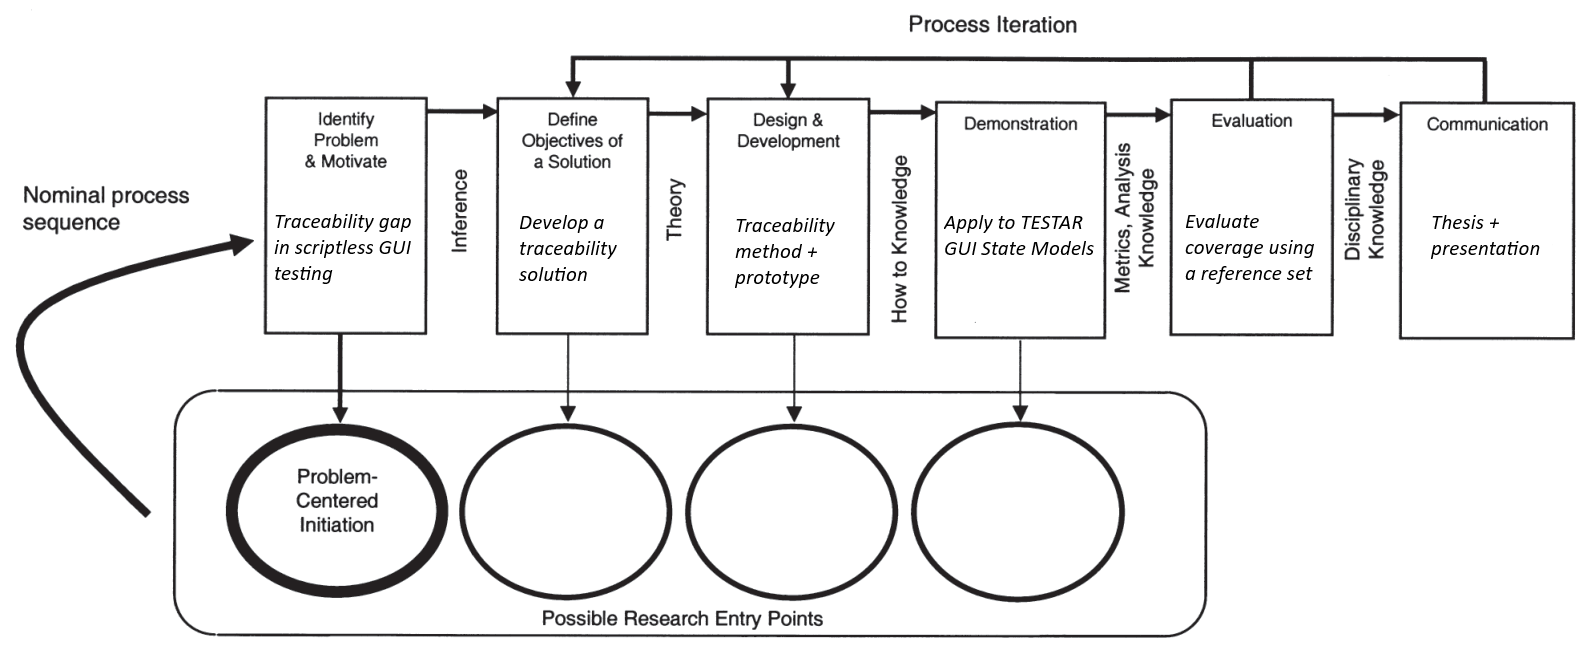
\includegraphics[width=0.95\textwidth]{dsrm-process-model}
    \caption{Adapted DSRM process model based on \citet{peffers2007design}.}
    \label{fig:dsrm-process-model}
\end{figure}

Figure~\ref{fig:dsrm-process-model} summarizes the adapted DSRM process model used to structure the research activities. The activities below list the main inputs and outputs. Identifiers refer to method components (A1--A4) and data and materials (D1--D5) defined later in this section.

\begin{description}
    \item[DSRM-A1 --- Problem identification and motivation:]
    Identify the traceability gap between user stories and test execution evidence in GUI State Models, and derive requirements for a solution. \\
    \textbf{Inputs:} user stories (D2), GUI State Models (D3). \\
    \textbf{Outputs:} problem statement, scope, solution requirements.

    \item[DSRM-A2 --- Define objectives of a solution:]
    Define design objectives and success criteria for story formalization, tracing, completeness assessment, and reporting. \\
    \textbf{Inputs:} outputs of DSRM-A1. \\
    \textbf{Outputs:} design objectives, evaluation criteria.

    \item[DSRM-A3 --- Design and development:]
    Design and implement the method and prototype, producing the main method components. \\
    \textbf{Inputs:} SUT configuration (D1), user stories (D2), GUI State Models (D3), scriptless GUI testing tool configuration (D4). \\
    \textbf{Outputs:} user story formalization (A1), tracing method (A2), completeness assessment (A3), prototype implementation (A4).

    \item[DSRM-A4 --- Demonstration:]
    Apply the prototype to GUI State Models to produce trace links and completeness outcomes and gather refinement feedback. \\
    \textbf{Inputs:} prototype (A4), user stories (D2), GUI State Models (D3). \\
    \textbf{Outputs:} traceability outputs, refinement feedback for A1--A4.

    \item[DSRM-A5 --- Evaluation:]
    Evaluate trace links and completeness outcomes against the reference set and analyze failure modes. \\
    \textbf{Inputs:} tracing method (A2), completeness assessment (A3), prototype (A4), GUI State Models (D3), reference set (D5). \\
    \textbf{Outputs:} evaluation results, failure-mode analysis.

    \item[DSRM-A6 --- Communication:]
    Document the method components, evaluation results, limitations, and implications. \\
    \textbf{Inputs:} outputs of DSRM-A1--A5. \\
    \textbf{Outputs:} thesis and supporting documentation.
\end{description}

\subsubsection{Method components}
\label{subsubsec:artifacts}

The traceability method consists of these components:

\begin{description}
    \item[A1 --- User story formalization:]
    A structured, machine-readable representation of user stories that makes required steps and expected UI outcomes explicit for analysis and matching.

    \item[A2 --- Tracing method:]
    A method to trace user story steps to test execution evidence in GUI State Models and to produce step-level trace links.

    \item[A3 --- Completeness assessment:]
    A method to assess user story execution completeness (not covered, partially covered, or fully covered) by aggregating step-level trace links.

    \item[A4 --- Prototype implementation:]
    A prototype implementation that applies A1--A3 to GUI State Models generated by TESTAR.
\end{description}

\subsubsection{Data and materials}
\label{subsubsec:data-materials}

The research uses these data and materials:

\begin{description}
    \item[D1 --- System Under Test (SUT) and configuration:]
    A selected SUT version and a documented test configuration (e.g., environment settings, test data accounts, and relevant preconditions) to support reproducible testing and model generation.

    \item[D2 --- User stories:]
    A set of functional requirements expressed as user stories for the selected SUT.

    \item[D3 --- GUI State Models:]
    One or more GUI State Models generated for the selected SUT using a scriptless GUI testing tool (TESTAR in this research). These models contain states, actions, and transitions and constitute the primary source of test execution evidence used for tracing and completeness assessment.

    \item[D4 --- Scriptless GUI testing tool and configuration:]
    The scriptless GUI testing tool used in this study, including the TESTAR version and the relevant exploration and logging settings.

    \item[D5 --- Reference set for evaluation:]
    A manually constructed reference set for a representative subset of stories and executions, including story-level completeness labels and, where applicable, step-level trace links.
\end{description}

\subsection{Validation}
\label{subsec:validation}

Validation assesses whether the proposed method and prototype address the research questions by evaluating their outputs on TESTAR-generated GUI State Models (D3). The evaluation uses a manually constructed reference set (D5) for a representative subset of stories and executions.

For tracing (RQ2), produced step-level trace links are compared to the reference set where available, complemented by targeted qualitative inspection of mismatches. For execution completeness (RQ3--RQ4), assessed user stories (not covered, partially covered, or fully covered) are compared to the reference labels in D5 and reported using standard multi-class metrics such as accuracy and macro-F1. In addition, failure-mode analysis is performed to characterize common sources of incorrect trace links or completeness outcomes.

The reference set (D5) will be created through manual inspection of the GUI State Models and, where available, supporting execution artifacts. Labeling decisions and assumptions will be documented; disagreements will be resolved through adjudication to make interpretation decisions explicit. When multiple GUI State Models are available (e.g., from different runs or configurations), results will be compared across models to assess robustness and sensitivity to testing settings.

Throughout the evaluation, \emph{not covered} is interpreted as \emph{not covered in the available GUI State Model evidence}, acknowledging that exploration coverage may limit what can be concluded from a given model.

\begin{table}[h!tb]
    \centering
    \caption{Validation approach aligned with research questions, method components, and required data.}
    \label{tab:validation}
    \begin{tabular}{p{1.6cm}p{3.4cm}p{3.6cm}p{6.0cm}}
        \toprule
        \textbf{RQ} & \textbf{Primary outputs} & \textbf{Required data} & \textbf{Validation approach} \\
        \midrule
        RQ1 & A1 & D2 & Check that stories can be represented consistently and are suitable for matching/tracing; spot-check on a representative subset. \\
        RQ2 & A2, A4 & D2, D3, D4, D5 & Compare produced trace links to the reference set where available; analyze mismatches and failure cases. \\
        RQ3 & A3, A4 & D3, D4, D5 & Compare assessed completeness labels to D5 (not covered/partially covered/fully covered); report multi-class metrics and inspect misclassifications. \\
        RQ4 & A1--A4 & D3, D5 & Evaluate overall effectiveness on TESTAR-generated models; report performance and failure-mode analysis; assess robustness across runs/configurations when available. \\
        \bottomrule
    \end{tabular}
\end{table}

\clearpage
% ====================================================
% Planning
% ====================================================
\section{Planning}
\label{sec:planning}

This section outlines the planning of the research activities described in Section~\ref{subsec:research-method}. The planning follows the Design Science Research Methodology (DSRM) activities (DSRM-A1--A6) and indicates how these activities are distributed over time.

The research is planned over twenty-one weeks. Although the activities are presented sequentially, the research process is iterative: insights from demonstration and evaluation may lead to refinements of earlier design decisions (e.g., adjustments to the structured story representation or tracing approach). Communication (writing) is continuous to ensure timely documentation of design decisions and results.

\begin{figure}[h!tb]
    \centering
    \resizebox{\textwidth}{!}{
        \begin{ganttchart}[
            hgrid,
            vgrid
        ]{1}{21}
            \gantttitle{Weeks}{21} \\
            \gantttitlelist{1,...,21}{1} \\

            \ganttbar{DSRM-A1: Problem identification and motivation}{1}{3} \\
            \ganttbar{DSRM-A2: Definition of solution objectives}{3}{5} \\
            \ganttbar{Data and materials preparation (D1--D4)}{4}{6} \\
            \ganttbar{DSRM-A3: Design and development}{6}{13} \\
            \ganttmilestone{Prototype implementation (A4)}{13} \\
            \ganttbar{DSRM-A4: Demonstration}{14}{16} \\
            \ganttbar{DSRM-A5: Evaluation}{17}{19} \\
            \ganttbar{DSRM-A6: Communication (thesis writing)}{6}{21} \\
            \ganttmilestone{Thesis submission}{21}
        \end{ganttchart}
    }
    \caption{Planning of the research activities aligned with the DSRM phases.}
    \label{fig:planning-gantt}
\end{figure}

\clearpage
% ====================================================
% Risk Analysis
% ====================================================
\section{Risk Analysis}
\label{sec:risk-analysis}

This section identifies key risks that may affect the design, implementation, and evaluation of the proposed method, and outlines mitigation measures. Likelihood and impact are assessed qualitatively as \emph{Low/Medium/High}.

\begin{description}
    \item[R1 --- Limited exploration coverage in GUI State Models:]
    GUI State Models (D3) may not cover all relevant user story steps due to the stochastic nature of scriptless exploration, leading to many stories being labeled \emph{not covered} even when the SUT supports the behavior. \\
    \textbf{Likelihood:} High. \\
    \textbf{Impact:} High. \\
    \textbf{Mitigation:} Run multiple explorations and/or configurations (D4) and aggregate evidence across models; clearly interpret \emph{not covered} as \emph{not covered in the available model evidence}; prioritize stories with observable UI effects.

    \item[R2 --- Ambiguity and variability in user story wording:]
    User stories (D2) may be underspecified, use domain-specific language, or describe outcomes not directly observable in the GUI State Model, reducing traceability. \\
    \textbf{Likelihood:} Medium. \\
    \textbf{Impact:} Medium. \\
    \textbf{Mitigation:} Define a structured representation (A1) with explicit step/outcome fields; introduce normalization rules and a glossary for key terms; document assumptions and handle ambiguous stories via documented interpretation rules.

    \item[R3 --- Incomplete or noisy model information:]
    GUI State Models may contain missing labels, unstable widget identifiers, duplicated states, or transitions that do not correspond cleanly to story steps, causing incorrect trace links (A2). \\
    \textbf{Likelihood:} Medium. \\
    \textbf{Impact:} High. \\
    \textbf{Mitigation:} Apply preprocessing and filtering (e.g., deduplication heuristics, label normalization); prefer robust features (e.g., action type + stable UI attributes); include failure-mode analysis in evaluation.

    \item[R4 --- Difficulty constructing a reliable reference set:]
    Manual creation of the reference set (D5) may be time-consuming and subject to disagreement, threatening evaluation validity. \\
    \textbf{Likelihood:} Medium. \\
    \textbf{Impact:} High. \\
    \textbf{Mitigation:} Limit D5 to a representative subset; use clear labeling guidelines; record rationale for labels; perform adjudication for disagreements; report inter-annotator agreement where feasible.

    \item[R5 --- Prototype implementation complexity and time constraints:]
    Integrating parsing, model access (e.g., graph database), tracing, and reporting in the prototype (A4) may exceed available time. \\
    \textbf{Likelihood:} Medium. \\
    \textbf{Impact:} High. \\
    \textbf{Mitigation:} Deliver a minimal end-to-end pipeline early; implement A1--A3 incrementally; timebox optional enhancements (e.g., advanced similarity/LLM support); keep interfaces modular so alternative tracing strategies can be swapped.

    \item[R6 --- Overfitting to a single SUT or configuration:]
    A method tuned to one SUT (D1) or one exploration configuration (D4) may not generalize. \\
    \textbf{Likelihood:} Medium. \\
    \textbf{Impact:} Medium. \\
    \textbf{Mitigation:} Evaluate on multiple runs/configurations where possible; include robustness checks; make design choices explicit and discuss external validity limitations.

    \item[R7 --- Threats to interpretability and reproducibility:]
    If parts of the tracing rely on heuristic thresholds or AI-based similarity, results may be harder to reproduce or explain. \\
    \textbf{Likelihood:} Medium. \\
    \textbf{Impact:} Medium. \\
    \textbf{Mitigation:} Prefer deterministic baselines; document parameters and thresholds; version-control code and configurations; report ablations (baseline vs enhanced strategy) when applicable.
\end{description}

\clearpage
% ====================================================
% Bibliography
% ====================================================
\bibliographystyle{plainnat}
\bibliography{report}

\end{document}
